\documentclass[12pt,oneside]{book}
\usepackage[utf8]{inputenc}
\usepackage[T1]{fontenc}
\usepackage{amsmath}
\usepackage{amsfonts}
\usepackage{amssymb}
\usepackage[none]{hyphenat}
\usepackage{geometry}
\usepackage{pdfpages}
\usepackage{graphicx}
\usepackage[titles]{tocloft}
\graphicspath{{images/}}
\usepackage{caption}
\usepackage{subcaption}
\usepackage{multicol}
\usepackage{multirow}
\usepackage{setspace}
\usepackage{algorithm}
\usepackage{float}
\usepackage{algorithmic}
\usepackage{enumitem}
\usepackage{natbib}
\usepackage{booktabs}
\bibliographystyle{abbrvnat}
\setcitestyle{authoryear,open={(},close={)}}
\usepackage[hidelinks]{hyperref}
\usepackage[printonlyused]{acronym}
\usepackage{listings}
\usepackage{xcolor}
\definecolor{codegreen}{rgb}{0,0.6,0}
\definecolor{codegray}{rgb}{0.5,0.5,0.5}
\definecolor{codepurple}{rgb}{0.58,0,0.82}
\definecolor{backcolour}{rgb}{0.95,0.95,0.92}
\lstdefinestyle{mystyle}{ %ref( https://www.overleaf.com/learn/latex/Code_listing )
	backgroundcolor=\color{backcolour},   
	commentstyle=\color{codegreen},
	keywordstyle=\color{magenta},
	numberstyle=\tiny\color{codegray},
	stringstyle=\color{codepurple},
	basicstyle=\ttfamily\footnotesize,
	breakatwhitespace=false,         
	breaklines=true,                 
	captionpos=b,                    
	keepspaces=true,                 
	numbers=left,                    
	numbersep=5pt,                  
	showspaces=false,                
	showstringspaces=false,
	showtabs=false,                  
	tabsize=2
}
\lstset{style=mystyle}

\begin{document}
%	\renewcommand{\arraystretch}{1.5}
%	\renewcommand{\baselinestretch}{0}
	\frontmatter
	
	\onehalfspacing

\begin{titlepage}
	\begin{center}
		
		\LARGE
		\textbf{GEORGIA STATE UNIVERSITY} \\
		Department of Mathematics and Statistics
		
		\vspace{0.35in}
		
		
\includegraphics[scale=0.3]{gsulogo}
		
		\vspace{0.5in}
		
		\textbf{METHODS FOR SOLVING INITIAL VALUE PROBLEMS - A Report}
		
		\vspace{0.8in}
		
		\large
		BY \\ \vspace{0.2in}
		JESSE ANNAN 
		
		\vspace{0.5in}
		April 15, 2023
		
	\end{center}
\end{titlepage}
		
	\tableofcontents
	
	\listofalgorithms
	
	\listoftables
	
	\listoffigures
	
	\addcontentsline{toc}{chapter}{LIST OF ABBREVIATIONS}
	\chapter*{List of Abbreviations}
	\begin{acronym}
	
	\acro{erc}[ERC]{Emotion Recognition in Conversation}
        \acro{adh}[ADH]{Autonomous Digital Human}
	\acro{iemocap}[IEMOCAP]{Interactive Emotional Dyadic Motion Capture}
	\acro{meld}[MELD]{Multimodal EmotionLines Dataset}
        \acro{bert}[BERT]{Bidirectional Encoder Representations from Transformers}
        \acro{cnn}[CNN]{Convolutional Neural Network}
        \acro{gru}[GRU]{Gated Recurrent Unit}
	\acro{cmt}[CMT]{Cross-Model Transformer}
        \acro{mtcnn}[MTCNN]{Multi-task Cascade Convolutional Network}
        \acro{mgif}[MGIF]{Multi-Grained Interactive Fusion}
        \acro{swfc}[SWFC]{Sample-Weighted Focal Constructive}

\end{acronym}

%%%%%%%%%%%%%%%%%%%%%%%%%%%%%%%%%%%%%%%%%%%%%%	
	\mainmatter
	
	\chapter{INTRODUCTION}
		\begin{spacing}{1.2}
			
			An \ac{ivp} is a \ac{de} together with one or more initial values.[\citenum{ryan}][\citenum{ivpwiki}] It takes what would otherwise be an entire rainbow of possible solutions and whittles them down to one specific solution. The basic idea behind this problem is that, once you differentiate a function, you lose some information about that function, more specifically, you lose the constant. By integrating $ y'(x) $, you get a family of solutions that only differ by a constant.[\citenum{krista}]
			
			\section{Definition}
				An \ac{ivp} is a differential equation: [\citenum{ivpwiki}]
				\begin{equation}
					\begin{split} \label{eq:ivp}
						y'(t) & = f(t, y(t)) \text{ with } f:\Omega \subset \mathbb{R} \times \mathbb{R}^n \rightarrow \mathbb{R}^n \\
						(t_{0}, y_{0}) & \in \Omega, \text{ called the initial condition.}
					\end{split}
				\end{equation}
				\subsection*{Observations: }
				\begin{enumerate}
					\item The given $ f $ in (\ref{eq:ivp}) is the defining function of \ac{ivp}.
					\item A unique solution, $ y(t) $, of the (\ref{eq:ivp}) exists and it satisfies $ y(t_{0}) = y_{0} $.
				\end{enumerate}
				
				\newpage
				
			\section*{Example}
				Given $ y'(t) = 5 $ and $ y(0) = -3 $, find $ y(t) $.
				\subsection*{Solution:}
					We first integrate our $ y'(t) $, then we substitute our initial condition to determine the constant (from our integration).
					\begin{equation*}
						\begin{split}
							\int y'(t) dt & = \int 5 dt \\
							 y(t) & = 5x + c \hspace*{0.3cm} \text{ where $ c $ is the constant of integration} \\
							 \text{using } y(t = 0) & = -3 \\
							 -3 & = 5(0) + c \\
							 -3 & = c \\
							 y(t) & = 2x - 3
						\end{split}
					\end{equation*}
					\textbf{Remark: } \text{Note that with a different $ y(0) $, the solution would be different.} 
			
			
			\section{Objective}
				In real-life situations, the differential equation that models a problem is too complicated to solve exactly, therefore one of the ways which is used to solved such problems is using methods which approximates the solution of the original problem.[\citenum{burden2015numerical}] In this report, I will discuss methods that approximates solutions at certain specified timestamps. \newline
				They are: [\S\ \ref{m:eul}] The Euler's Method, [\S\ \ref{m:meul}] The Modified Euler's Method, [\S\ \ref{m:rk2}] The 2nd-Order Runge-Kutta Method, [\S\ \ref{m:rk4}] The 4th-Order Runge-Kutta Method, \newline [\S\ \ref{m:ab4e}] The Adams-Bashforth 4th-Order Explicit, [\S\ \ref{m:ab4pc}] The Adams 4th-Order Predictor Corrector, [\S\ \ref{m:rkf}] The Runge-Kutta-Fehlberg, and [\S\ \ref{m:abpcvs}] The Predictor-Corrector methods
			
		\end{spacing}
		
	
	\chapter{METHODS}
	\section{The Euler's Method} \label{m:eul}
		\begin{spacing}{1.2}
			
			%\subsection{Introduction}
			The Euler method, named after Leonhard Euler, was published in his three-volume work \textit{Institutiones Calculi Integralis} in the years 1768 to 1770, and republished in his collected works.\citep{euler1913institutiones} [\citenum{butcher2016numerical}] The Euler method is a first-order numerical procedure for solving \ac{ode} with a given initial value. It is the most basic explicit method for numerical integration of \ac{ode} and is the simplest Runge–Kutta method.[\citenum{eulwiki}] \newline
			The fundamental idea of the method is based on the principle that, we can compute (or approximate) the shape of an unknown curve - in the form of a differential equation $ f(t,y) $, which starts at a given point $ y_{0} $ and time $ t_{0} $. With this information known, we can proceed to calculate the slope (tangent line) of the curve at $ y_{0} $. \newline
			The tangent line is [\citenum{eulpd}]
			\begin{equation*}
				y = y_{0} + f(t_{0}, y_{0}) \cdot (t - t_{0})
			\end{equation*}
			Now we assume that $ f(t0, y0) $ is sufficiently accurate, and thus, taking a small step along that tangent line, we can approximate the actual value of the solution, $ y_{1} $, at timestamp $ t_{1} $, using the formula:
			\begin{equation} \label{eqn:eul1}
				y_{1} = y_{0} + f(t_{0}, y_{0}) \cdot (t_{1} - t_{0})
			\end{equation}
			In general, we continue to find the next approximated solution $ y_{n+1} $ at $ t_{n+1} $, if we have the $ nth $ timestamp $ t_{n} $ and the approximation to the solution at this point, $ y_{n} $. We only need to modify (\ref{eqn:eul1}) in this manner:
			\begin{equation} \tag{2.2a}
				y_{n+1} = y_{n} + f(t_{n}, y_{n}) \cdot (t_{n+1} - t_{n})
			\end{equation}
			If we assume uniform step sizes between times, $ t $, we can define, $ h = t_{n+1} - t_{n} $. Therefore, the formula is simplified as [\citenum{eulpd}]
			\begin{equation} \label{eqn:eul} \tag{2.2b}
				y_{n+1} = y_{n} + h \cdot f(t_{n}, y_{n})
			\end{equation}
			
			\subsection*{The Truncation Errors}
				\begin{enumerate}
					\item The \textbf{\ac{lte}} of the Euler method is the error made in a single step. It is the difference between the numerical solution after one step, $y_{1}$, and the exact solution (obtained using Taylor's expansion) at time $t_{1} = t_{0} + h$.[\citenum{eulwiki}]
					\begin{equation*}
						\begin{split}
							\text{The numerical solution: } y_{1} & = y_{0} + hf(t_{0}, y_{0}) \\
							\text{The exact solution: } y(t_{0} + h) & = y(t_{0}) + hy'(t_{0}) + \frac{1}{2}h^2y^{''}(t_{0}) + O(h^{3}) \\
							\ac{lte} & = y(t_{0} + h) - y_{1} = \frac{1}{2}h^2y^{''}(t_{0}) + O(h^{3})
						\end{split}
					\end{equation*}
					
					\item The \textbf{\ac{gte}} is the error at a fixed time $t_{i}$, after however many steps the method needs to take to reach that time from the initial time. The global truncation error is the cumulative effect of the local truncation errors committed in each step.[\citenum{atkinson1991introduction}]
					\begin{equation*}
						|y(t_{i}) - y_{i}| \leq \frac{hM}{2L} (e^{L(t_{i} - t_{0})} - 1)
					\end{equation*}
					where $ M $ is an upper bound on the second derivative of y on the given interval and $ L $ is the Lipschitz constant of $ f $.[\citenum{atkinson1991introduction}]
				\end{enumerate}
			
			\subsection*{The Pseudocode}
				To approximate the solution of the \ac{ivp}
				\[ y' = f(t,y), \hspace*{0.2cm} a \leq t \leq b, \hspace*{0.2cm} y(a) = \alpha \]
				at $ N $ equally spaced numbers in the interval $ [a, b]: $ [\citenum{burden2015numerical}]
				
				\begin{algorithm}[H]
					\caption{:: Euler's Method}
					\begin{algorithmic}[1]
						\REQUIRE endpoints $ a, b $; \hspace*{0.2cm} integer $ N $; \hspace*{0.2cm} initial condition $ \alpha $
						\ENSURE approximation $ w $ to $ y $ at the $ (N + 1) $ values of $ t $
						\STATE $ h = (b - a) / N; \hspace*{0.2cm} t_0 = a; \hspace*{0.2cm} w_{0} = \alpha $
						\FOR{$ i = 0, 1, 2, \cdots, N-1$}
							\STATE $ w_{i+1} = w_{i} + hf(t_{i},w_{i}); $ \hspace*{0.5cm} \COMMENT{Compute next $ w_{i} $}
							\STATE $ t = a + ih $ \hspace*{0.5cm} \COMMENT{Compute next $ t_{i} $}
						\ENDFOR
						\RETURN $ (t, w) $
					\end{algorithmic}
				\end{algorithm}
			
		\end{spacing}

	\clearpage
	\section{The Modified Euler's Method} \label{m:meul}
		\begin{spacing}{1.2}
			
			%\subsection{Introduction}
			Euler's method is used as the foundation for Modified Euler's method. Euler's method uses the line tangent to the function at the beginning of the interval as an estimate of the slope of the function over the interval, assuming that if the step size is small, the error will be small. However, even when extremely small step sizes are used, over a large number of steps the error starts to accumulate and the estimate diverges from the actual functional value.[\citenum{heulwiki}] \newline
			The Modified Euler (which may sparingly be referred to as the Heun's method [\citenum{heulwiki}]) was developed to improve the approximated solution at $t_{i+1}$ by taking the arithmetic average of the approximated solution at the slopes $t_{i}$ and $t_{i+1}$. \newline
			The procedure for calculating the numerical solution to the (\ref{eq:ivp}) by first computing the Euler method to roughly estimate the coordinates of the next point in the solution, and then, the original estimate is recalculated using the rough estimate [\citenum{chenadvanced}]:
				\begin{equation}
					\begin{split}
						\text{rough estimate: } \tilde{y}_{i+1} & = y_{i} + hf(t_{i}, y_{i}) \\
						\text{original estimate: } y_{i+1} & = y_{i} + \frac{h}{2} \left[f(t_{i}, y_{i}) + f(t_{i+1}, \tilde{y}_{i+1}) \right]
					\end{split}
				\end{equation}
				where $ h $ is the step size an $ t_{i+1} = t_{i} + h. $
			
			\subsection*{The Truncation Errors}
				The local truncation error is $ O(h^{3}) $. The modified Euler Method is second order accurate.
			
			\clearpage
			\subsection*{The Pseudocode}
				To approximate the solution of the \ac{ivp} 
				\[ y' = f(t,y), \hspace*{0.2cm} a \leq t \leq b, \hspace*{0.2cm} y(a) = \alpha \]
				at $ N $ equally spaced numbers in the interval $ [a, b]: $
				
				\begin{algorithm}[H]
					\caption{:: Modified Euler's Method}
					\begin{algorithmic}[1]
						\REQUIRE endpoints $ a, b $; \hspace*{0.2cm} integer $ N $; \hspace*{0.2cm} initial condition $ \alpha $
						\ENSURE approximation $ w $ to $ y $ at the $ N $ values of $ t $
						\STATE $ h = (b - a) / N; \hspace*{0.2cm} t_0 = a; \hspace*{0.2cm} w_{0} = \alpha $
						\FOR{$ i = 0, 1, 2, \cdots, N-1$}
							\STATE $ \tilde{w}_{i+1} = w_{i} + hf(t_{i},w_{i}); $ \hspace*{0.5cm} \COMMENT{Compute rough (next) $ w_{i} $}
							\STATE $ w_{i+1} = w_{i} + \frac{h}{2} \left[ f(t_{i},w_{i}) + f(t_{i} + h,\tilde{w}_{i+1}) \right]; $ \hspace*{0.5cm} \COMMENT{Compute corrected (next) $ w_{i} $}
							\STATE $ t = a + ih $ \hspace*{0.5cm} \COMMENT{Compute next $ t_{i} $}
						\ENDFOR
						\RETURN $ (t, w) $
					\end{algorithmic}
				\end{algorithm}
			
		\end{spacing}
		
	\clearpage
	\section{The 2nd-Order Runge-Kutta Method} \label{m:rk2}
		\begin{spacing}{1.2}
			
			%\subsection{Introduction}
			The Runge-Kutta methods have the higher-order local truncation error of the Taylor methods while eliminating the need to compute and evaluate the derivative of $ f(t, y) $. The \ac{rk2} is one of the methods that computes the approximation of $ y $ for a given timestamp. The \ac{rk2} can only be used to used to solve first-order ordinary differential equations. This is done by computing, $ k_{1} $, the increment based on the slopes at the beginning of the interval using $ y $ and $ k_2 $, the increment based on the slope at the midpoint of the interval, using $ (y + \frac{h}{2}k_{1}) $ [\citenum{rk2geek}]
			\begin{equation} \label{eq:rk2}
				\begin{split}
					w_{0} & = \alpha \\
					k_{1} & = f(t_{i},w_{i}) \\
					k_{2} & = f\left(t_{i} + \frac{h}{2}, w_{i} + \frac{h}{2}k_{1}\right); \\
					w_{i+1} & = w_{i} + hk_{2} \hspace*{0.5cm} \forall i = 0, 1, \cdots, N - 1
				\end{split}
			\end{equation}
			
			\subsection*{The Truncation Errors}
				The method is a second-order method, meaning that the local truncation error is in the order of $ O(h^3) $, while the total accumulated error is order of $ O(h^4) $.[\citenum{rk2geek}]
			
			\clearpage
			\subsection*{The Pseudocode}
				To approximate the solution of the \ac{ivp} 
				\[ y' = f(t,y), \hspace*{0.2cm} a \leq t \leq b, \hspace*{0.2cm} y(a) = \alpha \]
				at $ N $ equally spaced numbers in the interval $ [a, b]: $
				
				\begin{algorithm}[H]
					\caption{:: \ac{rk2}}
					\begin{algorithmic}[1]
						\REQUIRE endpoints $ a, b $; \hspace*{0.2cm} integer $ N $; \hspace*{0.2cm} initial condition $ \alpha $
						\ENSURE approximation $ w $ to $ y $ at the $ N $ values of $ t $
						\STATE $ h = (b - a) / N; \hspace*{0.2cm} t_0 = a; \hspace*{0.2cm} w_{0} = \alpha $
						\FOR{$ i = 0, 1, 2, \cdots, N-1$}
							\STATE $ k_{1} = f(t_{i},w_{i}); $ \hspace*{0.5cm} \COMMENT{Compute $ k_{1} $}
							\STATE $ k_{2} = f\left(t_{i} + \frac{h}{2}, w_{i} + \frac{h}{2}k_{1}\right); $ \hspace*{0.5cm} \COMMENT{Compute $ k_{2} $}
							\STATE $ w_{i+1} = w_{i} + hk_{2}; $ \hspace*{0.5cm} \COMMENT{Compute next $ w_{i} $}
							\STATE $ t = a + ih $ \hspace*{0.5cm} \COMMENT{Compute next $ t_{i} $}
						\ENDFOR
						\RETURN $ (t, w) $
					\end{algorithmic}
				\end{algorithm}
			
		\end{spacing}
		
		\clearpage
	\section{The 4th-Order Runge-Kutta Method} \label{m:rk4}
		\begin{spacing}{1.2}
			
			%\subsection{Introduction}
			(\ref{eq:rk2}) can be extended to higher order methods. The \ac{rk4} is another scheme of the Runge-Kutta methods. This methods involves computing four increments $ k_{1,2,3,4} $ (instead of two done above by \ac{rk2}). Each increment is the product of the size of the interval, $ h $. $ k_{1} $ is the slope at the beginning of the interval, using $ y $ (similar to Euler's method), $ k_{2} $ is the slope at the midpoint of the interval, using the $ y \text{ and } k_{1}$, $ k_{3} $ is the slope at the midpoint, using $ y \text{ and } k_{2} $ and finally the forth $ k $, $ k_{4} $ is the slope at the end of the interval, using $ y \text{ and } k_{3} $.[\citenum{rkwiki}]
			\begin{equation} \label{eq:rk4}
				\begin{split}
					k_{1} & = f(t_{i},w_{i}) \\
					k_{2} & = f\left(t_{i} + \frac{h}{2}, w_{i} + \frac{h}{2}k_{1}\right); \\
					k_{3} & = f\left(t_{i} + \frac{h}{2}, w_{i} + \frac{h}{2}k_{2}\right); \\
					k_{4} & = f\left(t_{i} + h, w_{i} + hk_{3}\right); \\
					w_{i+1} & = w_{i} + \frac{h}{6} ( k_{1} + 2k_{2} + 2k_{3} + k_{4} );
				\end{split}
			\end{equation}
			
			\subsection*{The Truncation Errors}
				Since \ac{rk4} needs to evaluate the function $ f $ for four times in each step meaning the local truncation error is on the order of $ O(h^{5}) $, while the total accumulated error is on the order of $ O(h^{4}) $.[\citenum{rkwiki}]
			
			\clearpage
			\subsection*{The Pseudocode}
				To approximate the solution of the \ac{ivp} 
				\[ y' = f(t,y), \hspace*{0.2cm} a \leq t \leq b, \hspace*{0.2cm} y(a) = \alpha \]
				at $ N $ equally spaced numbers in the interval $ [a, b]: $ [\citenum{burden2015numerical}]
				
				\begin{algorithm}[H]
					\caption{:: \ac{rk4}}
					\begin{algorithmic}[1]
						\REQUIRE endpoints $ a, b $; \hspace*{0.2cm} integer $ N $; \hspace*{0.2cm} initial condition $ \alpha $
						\ENSURE approximation $ w $ to $ y $ at the $ N $ values of $ t $
						\STATE $ h = (b - a) / N; \hspace*{0.2cm} t_0 = a; \hspace*{0.2cm} w_{0} = \alpha $
						\FOR{$ i = 0, 1, 2, \cdots, N-1$}
						\STATE $ k_{1} = f(t_{i},w_{i}); $ \hspace*{0.5cm} \COMMENT{Compute $ k_{1} \; to \; k_{4} $}
						\STATE $ k_{2} = f\left(t_{i} + \frac{h}{2}, w_{i} + \frac{h}{2}k_{1}\right); $
						\STATE $ k_{3} = f\left(t_{i} + \frac{h}{2}, w_{i} + \frac{h}{2}k_{2}\right); $
						\STATE $ k_{4} = f\left(t_{i} + h, w_{i} + hk_{3}\right); $
						\STATE $ K = k_{1} + 2k_{2} + 2k_{3} + k_{4}  $
						\STATE $ w_{i+1} = w_{i} + \frac{h}{6}K; $ \hspace*{0.5cm} \COMMENT{Compute next $ w_{i} $}
						\STATE $ t = a + ih $ \hspace*{0.5cm} \COMMENT{Compute next $ t_{i} $}
						\ENDFOR
						\RETURN $ (t, w) $
					\end{algorithmic}
				\end{algorithm}
			
		\end{spacing}
		
		\clearpage
	\section{The Adams-Bashforth 4th-Order Explicit Method} \label{m:ab4e}
		\begin{spacing}{1.2}
			
			%\subsection{Introduction}
			Adams-Bashforth 4th Order Explicit Method is a member of the Adams-Bashforth family of explicit numerical methods that approximates the solution of an IVP by using a weighted average of previous function values. This method is useful when the function evaluations are relatively cheap and the derivative is known explicitly.  The scheme for Adams-Bashforth explicit methods of order 4 is:[\citenum{burden2015numerical}]			
			\begin{equation}
				\begin{split}
					w_0 & = \alpha \\
					w_1 & = \alpha_1 \\
					w_2 & = \alpha_2 \\
					w_3 & = \alpha_3 \\
					w_{i+1} & = w_{i} + \frac{h}{24}[ 55f(t_{i} - h, w_{i}) - 59f(t_{i-1} - h, w_{i-1}) \\
					& + 37f(t_{i-2} - h, w_{i-2}) - 9f(t_{i-3} - h, w_{i-3}) ] \\
					\text{where } i & = 3, 4, ..., N-1
				\end{split}
			\end{equation}
			
			\subsection*{The Truncation Errors}
				The Adams-Bashforth 4th-Order Explicit Method local truncation error is [\citenum{burden2015numerical}] \[ \tau_{i+1}(h) = \frac{251}{720} y^{5}(\mu_{i}) h^{4} \]
				for some $ \mu_{i} \in (t_{i-3}, t_{i+1}) $
			
			\clearpage
			\subsection*{The Pseudocode}
				To approximate the solution of the \ac{ivp} 
				\[ y' = f(t,y), \hspace*{0.2cm} a \leq t \leq b, \hspace*{0.2cm} y(a) = \alpha \]
				at $ N $ equally spaced numbers in the interval $ [a, b]: $ [\citenum{burden2015numerical}]
				
				\begin{algorithm}[H]
					\caption{:: Adams-Bashforth 4th-Order Explicit Method}
					\begin{algorithmic}[1]
						\REQUIRE endpoints $ a, b $; \hspace*{0.2cm} integer $ N $; \hspace*{0.2cm} initial condition $ \alpha $
						\ENSURE approximation $ w $ to $ y $ at the $ N $ values of $ t $
						\STATE Compute the first 3 values for $ t_{i} $ and $ w_{i} $ using the $ RK4 $ method
						\STATE Call $ RK4 $ \hspace*{0.5cm} \COMMENT{ \ac{rk4} method above }
						\STATE $ h = (b - a) / N; \hspace*{0.2cm} t_0 = a; \hspace*{0.2cm} w_{0} = \alpha $
						\FOR{$ i = 3, 4, 5, \cdots, N-1$}
						\STATE $ k_{1} = f(t_{i},w_{i}); $ \hspace*{0.5cm} \COMMENT{Compute $ k_{1} \; to \; k_{4} $}
						\STATE $ k_{2} = f(t_{i} - h, w_{i-1}); $
						\STATE $ k_{3} = f(t_{i} - 2h, w_{i-2}); $
						\STATE $ k_{4} = f(t_{i} - 3h, w_{i-3}); $
						\STATE $ K = 55k_{1} - 59k_{2} + 37k_{3} - 9k_{4}  $
						\STATE $ w_{i+1} = w_{i} + \frac{h}{24}K; $ \hspace*{0.5cm} \COMMENT{Compute next $ w_{i} $}
						\STATE $ t = a + ih $ \hspace*{0.5cm} \COMMENT{Compute next $ t_{i} $}
						\ENDFOR
						\RETURN $ (t, w) $
					\end{algorithmic}
				\end{algorithm}
			
		\end{spacing}
		
		\clearpage
	\section{The Adams 4th-Order Predictor-Corrector Method} \label{m:ab4pc}
		\begin{spacing}{1.2}
			
			%\subsection{Introduction}
			The methods discussed above only involves predicting the approximate solution just ones. The Adams-Bashforth 4th-Order Explicit Method is one of the many multi-stage methods. The method involves the combination of an explicit and implicit technique and is called a predictor-corrector method. [\citenum{burden2015numerical}] The explicit method predicts an approximation, and the implicit method corrects this prediction. \newline
			Consider the (\ac{ivp}) stated above. The first step is to calculate the starting values $ w_{0}, w_{1}, w_{2} \text{ and } w_{3} $ for the four-step explicit Adams-Bashforth method. This is done by using the Runge-Kutta 4th-order method, then approximate the immediate $ w_{i} $  using the explicit Adams-Bashforth. The approximation is then improved in the next step using the three-step impplicit Adams-Moulton method: [\citenum{burden2015numerical}]
			\begin{equation}
				\begin{split}
					\text{Predict $ w_{i} $: } w_{p} & = w_{3} + h [ 55f(t_{3}. w_{3}) - 59f(t_{2}, w_{2}) \\
					& \hspace*{0.5cm} + 37f(t_{1}, w_{1}) - 9f(t_{0}, w_{0}) ] / 24; \\
					\text{Correct $ w_{i} $: } w_{c} & = w_{3} + h [ 9f(t_{i+1}. w_{i+1}) - 19f(t_{3}, w_{3}) \\
					& \hspace*{0.5cm} - 5f(t_{2}, w_{2}) + f(t_{1}, w_{1}) ] / 24;
				\end{split}
			\end{equation}
			
			\subsection*{The Truncation Errors}
			The Adams 4th-Order Predictor-Corrector Method has an error order of $ O(h^4) $. [\citenum{burden2015numerical}]	
			
			
			\subsection*{The Pseudocode}
				To approximate the solution of the \ac{ivp} 
				\[ y' = f(t,y), \hspace*{0.2cm} a \leq t \leq b, \hspace*{0.2cm} y(a) = \alpha \]
				at $ N $ equally spaced numbers in the interval $ [a, b]: $ [\citenum{burden2015numerical}]
				
				\begin{algorithm}[H]
					\caption{:: Adams Forth-Order Predictor-Corrector}
					\begin{algorithmic}[1]
						\REQUIRE endpoints $ a, b $; \hspace*{0.2cm} integer $ N $; \hspace*{0.2cm} initial condition $ \alpha $
						\ENSURE approximation $ w $ to $ y $ at the $ N $ values of $ t $
						\STATE $ h = (b - a) / N $
						\STATE $ t_0 = a $
						\STATE $ w_0 = \alpha $
						\FOR{$ i = 0, 1, 2 $}
							\STATE $ k_1 = hf(t_{i}, w_{i}); $ \COMMENT{Compute starting values using Runge-Kutta Method}
							\STATE $ k_2 = hf(t_{i} + \frac{h}{2}, w_{i} + \frac{k_{1}}{2}); $
							\STATE $ k_3 = hf(t_{i} + \frac{h}{2}, w_{i} + \frac{k_{2}}{2}); $
							\STATE $ k_4 = hf(t_{i} + h, w_{i} + k_{3}); $
							\STATE $ K = k_{1} + 2k_{2} + 2k_{3} + k_{4} $
							\STATE $ w_{i+1} = w_{i} + \frac{K}{6}; $
							\STATE $ t_{i+1} = a + ih $
							\RETURN $ (t_{i}, w_{i}) $
						\ENDFOR
						\FOR{$ i = 3, \cdots, N-1 $}
							\STATE $ t = a + ih; $
							\STATE $ w_{i+1} = w_{3} + h \frac{[ 55f(t_{3}. w_{3}) - 59f(t_{2}, w_{2}) + 37f(t_{1}, w_{1}) - 9f(t_{0}, w_{0}) ]}{24}; $ \COMMENT{Predict $ w_{i+1} $}
							\STATE $ w_{i+1} = w_{3} + h \frac{[ 9f(t_{i+1}. w_{i+1}) - 19f(t_{3}, w_{3}) - 5f(t_{2}, w_{2}) + f(t_{1}, w_{1}) ]}{24}; $ \COMMENT{Correct $ w_{i+1} $}
							\RETURN $ (t, w) $
							\FOR{$ j = 0, 1, 2 $}
								\STATE $ t_{j} = t_{j+1}; $
								\STATE $ w_{j} = w_{j+1} $
							\ENDFOR
							\STATE $ t_{3} = t_{i+1}; $
							\STATE $ w_{3} = w_{i+1} $
						\ENDFOR
					\end{algorithmic}
				\end{algorithm}
			
		\end{spacing}
		
		\clearpage
	\section{The Runge-Kutta-Fehlberg Method} \label{m:rkf}
		\begin{spacing}{1.2}
			
			%\subsection{Introduction}
			The Runge–Kutta–Fehlberg method (or Fehlberg method) is an algorithm in numerical analysis for the numerical solution of ordinary differential equations. It was developed by the German mathematician Erwin Fehlberg and is based on the large class of Runge–Kutta methods.
			The novelty of Fehlberg's method is that it is an embedded method from the Runge–Kutta family, meaning that identical function evaluations are used in conjunction with each other to create methods of varying order and similar error constants.[\citenum{rkfmatlab}] The \ac{rkf} method is used for error control because at each step it provides, at little additional cost, two approximation that can be compared and related to the local error.[\citenum{burden2015numerical}]
			\begin{equation}
				\begin{split}
					k_1 & = hf(t,w); \\
					k_2 & = hf(t + \frac{1}{4}h, w + \frac{1}{4}k_1); \\
					k_3 & = hf(t + \frac{3}{8}h, w + \frac{3}{32}k_1 + \frac{9}{32}k_2); \\ 
					k_4 & = hf(t + \frac{12}{13}h, w + \frac{1932}{2197}k_1 - \frac{7200}{2197}k_2 + \frac{7296}{2197}k_3); \\ 
					k_5 & = hf(t + h, w + \frac{439}{216}k_1 - 8k_2 + \frac{3680}{513}k_3 - \frac{845}{4104}k_4); \\
					k_6 & = hf(t + \frac{1}{2}h, w - \frac{8}{27}k_1 + 2k_2 - \frac{3544}{2565}k_3 + \frac{1859}{4104}k_4 - \frac{11}{40}k_5);
				\end{split}
			\end{equation}
			
			\subsection*{The Truncation Errors}
				It can be shown that the first formula is an O(h5) while the second is $ O(h^6) $ (though only $ O(h^4) $ and $ O(h^5) $. [\citenum{rkfwat}]
			
			\subsection*{The Pseudocode} 
				To approximate the solution of the \ac{ivp}  $ y' = f(t,y), \hspace*{0.2cm} a \leq t \leq b, \hspace*{0.2cm} y(a) = \alpha $
				with local truncation error within a given tolerance: [\citenum{burden2015numerical}]
				
				\begin{algorithm}[H]
					\caption{:: \ac{rkf}}
					\begin{algorithmic}[1]
						\REQUIRE endpoints $ a, b $; \hspace*{0.2cm} a tolerance $ TOL $; \hspace*{0.2cm} initial condition $ \alpha $ \hspace*{0.2cm} maximum step size $ hmax $; \hspace*{0.2cm} minimum step size $ hmin $
						\ENSURE $ t, w, h $ where $ w $ approximates $ y(t) $ and the step size $ h $ was used, or a message that the minimum step size was exceeded.
						\STATE $ t = a; \hspace*{0.2cm} w = \alpha; \hspace*{0.2cm} h = hmax; Flag=1; $
						\WHILE{$ Flag==1 $}
							\STATE $ k_1 = hf(t,w); $
							\STATE $ k_2 = hf(t + \frac{1}{4}h, w + \frac{1}{4}k_1); $
							\STATE $ k_3 = hf(t + \frac{3}{8}h, w + \frac{3}{32}k_1 + \frac{9}{32}k_2); $
							\STATE $ k_4 = hf(t + \frac{12}{13}h, w + \frac{1932}{2197}k_1 - \frac{7200}{2197}k_2 + \frac{7296}{2197}k_3); $
							\STATE $ k_5 = hf(t + h, w + \frac{439}{216}k_1 - 8k_2 + \frac{3680}{513}k_3 - \frac{845}{4104}k_4); $
							\STATE $ k_6 = hf(t + \frac{1}{2}h, w - \frac{8}{27}k_1 + 2k_2 - \frac{3544}{2565}k_3 + \frac{1859}{4104}k_4 - \frac{11}{40}k_5); $
							\STATE $ R = \frac{1}{h} | \frac{1}{360}k_1 - \frac{128}{4275}k_3 - \frac{2197}{75240}k_4 + \frac{1}{50}k_5 + \frac{2}{55}k_6 | $ \hspace*{0.5cm} \COMMENT{Note: $ R = \frac{1}{h} | \tilde{w}_{i+1} - w_{i+1} | $}
							\IF{$ R \leq TOL $}
								\STATE $ t = t + h; $
								\STATE $ w = w + \frac{25}{216}k_1 + \frac{1408}{2565}k_3 + \frac{2197}{4104}k_4 - \frac{1}{5}k_5 $
								\RETURN $ (t, w, h) $
							\ENDIF
							\STATE $ \delta = 0.84 (TOL/R)^{\frac{1}{4}} $
							\IF{$ \delta \leq 0.1 $} 
								\STATE $ h = 0.1h $\hspace*{0.5cm} \COMMENT{Calculate new $ h $}
							\ELSIF{$ \delta \geq 4 $}
								\STATE $ h = 4h $
							\ELSE
								\STATE $ h = \delta h $
							\ENDIF
							\IF{$ h > hmax $}
								\STATE $ h = hmax $
							\ENDIF
							\IF{$ t \geq b $}
								\STATE $ Flag = 0 $
							\ELSIF{$ t + h > b $}
								\STATE $ h = b - t $
							\ELSIF{$ h < hmin $}
								\STATE $ Flag = 0 $
								\PRINT "minimum $ h $ exceeded" \hspace*{0.5cm} \COMMENT{Procedure completed unsuccessfully}
							\ENDIF
						\ENDWHILE
						\RETURN $ (t, w) $
					\end{algorithmic}
				\end{algorithm}
			
		\end{spacing}
		
		\clearpage
	\section{The Adams Variable Step-Size Predictor-Corrector} \label{m:abpcvs}
		\begin{spacing}{1.2}
			
			%\subsection{Introduction}
			The Adams Variable Step-Size Predictor-Corrector is another variable step-size multistep method. Instead of producing two approximation that can be compared and related to the local error, the predictor-corrector techniques always generate two approximation at each step, so they are naturally candidates for error-control adaptation.[\citenum{burden2015numerical}] \newline
			The Adams Variable Step-Size Predictor-Corrector uses the four-step explicit Adams Bashforth method as predictor and the three-step implicit Adams-Moulton method as corrector.[\citenum{burden2015numerical}]
			\begin{equation}
				\begin{split}
					\text{Predictor $ y_{t_{i+1}} $: } y_{p} & = y_{t_i} + \frac{h}{24} [ 55f(t_{i}. y_{t_i}) - 59f(t_{i-1}, y_{t_{i-1}}) \\
					& \hspace*{0.5cm} + 37f(t_{i-2}, y_{t_{i-2}}) - 9f(t_{i-3}, y_{t_{i-3}}) ] + \frac{251}{720}y^{(5)}(\hat{\mu}_i)h^5; \\
					\text{Corrector $ y_{t_{i+1}} $: } w_{c} & = y_{t_i} + \frac{h}{24} [ 9f(t_{i+1}. y_{t_{i+1}}) - 19f(t_{i}. y_{t_{i}}) \\
					& \hspace*{0.5cm} - 5f(t_{i-1}. y_{t_{i-1}}) + f(t_{i-2}. y_{t_{i-2}}) ] - \frac{19}{720}y^{(5)}( \tilde{\mu}_i)h^4;
				\end{split}
			\end{equation}
			
			%\subsection*{The Truncation Errors}
			
			\subsection*{The Pseudocode}
				To approximate the solution of the \ac{ivp} 
				\[ y' = f(t,y), \hspace*{0.2cm} a \leq t \leq b, \hspace*{0.2cm} y(a) = \alpha \]
				with local truncation error within a given tolerance: [\citenum{burden2015numerical}]
				
				\begin{algorithm}[H]
					\caption{:: Adams Variable Step-Size Predictor-Corrector}
					\begin{algorithmic}[1]
						\REQUIRE endpoints $ a, b $; \hspace*{0.2cm} a tolerance $ TOL $; \hspace*{0.2cm} initial condition $ \alpha $ \hspace*{0.2cm} maximum step size $ hmax $; \hspace*{0.2cm} minimum step size $ hmin $
						\ENSURE $ t, w, h $ where $ w $ approximates $ y(t) $ and the step size $ h $ was used, or a message that the minimum step size was exceeded.
						\STATE \COMMENT{Set up a subalgorithm for the Runge-Kutta 4th-Order method to be called $ RK4(h, v_{0}, x_{0}, v_{1}, x_{1}, v_{2}, x_{2}, v_{3}, x_{3}) $ that accepts as input a step size $ h $ and starting values $ v_{0} \approx y(t_{0}) $ and returns $ \{ (x_{j}, v_{j}) | j = 1, 2, 3 \} $ defined by the following:}
						\FOR{$ j = 1, 2, 3 $}
							\STATE $ k_{1} = hf(x_{j-1}, v_{j-1}); $
							\STATE $ k_{2} = hf(x_{j-1} + \frac{h}{2}, v_{j-1} + \frac{k_{1}}{2}); $
							\STATE $ k_{3} = hf(x_{j-1} + \frac{h}{2}, v_{j-1} + \frac{k_{2}}{2}); $
							\STATE $ k_{4} = hf(x_{j-1} + h, v_{j-1} + k_{3}); $
							\STATE $ K = k_{1} + 2k_{2} + 2k_{3} + k_{4} $
							\STATE $ v_{j} = v_{j-1} + \frac{K}{6}; $
							\STATE $ x_{j} = x_{0} + jh $
						\ENDFOR
						\STATE $ t_{0} = a; $
						\STATE $ w_{0} = \alpha; $
						\STATE $ h = hmax; $
						\STATE $ Flag = 1 $ \hspace*{0.5cm} \COMMENT{$ Flag $ will be used to exit a loop.}
						\STATE $ Last = 0 $ \hspace*{0.5cm} \COMMENT{$ Last $ will indicate when the last value is calculated.}
						\STATE Call $ RK4(h, v_{0}, x_{0}, v_{1}, x_{1}, v_{2}, x_{2}, v_{3}, x_{3}) $
						\STATE $ Nflag = 1; $ \hspace*{0.5cm} \COMMENT{Indicates computation from $ RK4 $}
						\STATE $ i = 4; $
						\STATE $ t = t_{3} + h $
						\WHILE{$ Flag == 1 $}
							\STATE $ w_{p} = w_{i-1} + \frac{h}{24} [ 55f(t_{i-1}, w_{i-1}) - 59f(t_{i-2}, w_{i-2}) + 37f(t_{i-3}, w_{i-3}) - 9f(t_{i-4}, w_{i-4}); ] $ \hspace*{0.5cm} \COMMENT{Predict $ w_{i} $}
							\STATE $ w_{c} = w_{i-1} + \frac{h}{24} [ 9f(t, w_{p}) + 19f(t_{i-1}, w_{i-1}) - 5f(t_{i-2}, w_{i-2}) + f(t_{i-3}, w_{i-3}); ] $ \hspace*{0.5cm} \COMMENT{Correct $ w_{i} $}
							\STATE $ \sigma = 19 | w_{c} - w_{p} | / 270h $
							\STATE $ \vdots $
							\STATE $ \vdots $ \COMMENT{next page}
							\STATE $ \vdots $
%							\IF{$ \sigma \leq TOL $}
%								\STATE $ w_{i} = w_{c} $ \hspace*{0.5cm} \COMMENT{Result accepted}
%								\STATE $ t_{i} = t $
%								\IF{$ Nflag == 1 $}
%									\FOR{$ j = i-3, i-2, i-1, i $}
%										\RETURN $ (j, t_{j}, w_{j}, h); $ \hspace*{0.5cm} \COMMENT{Previous results also accepted}
%									\ENDFOR
%								\ELSE
%									\RETURN $ (i, t_{i}, w_{i}, h) $ \hspace*{0.5cm} \COMMENT{Previous results already accepted}
%								\ENDIF
%								\IF{$ Last == 1 $}
%									\STATE $ Flag = 0 $
%								\ELSE %10-16
%									\STATE $ i = i + 1 $
%									\STATE $ Nflag = 0 $
%									\IF{$ \sigma \leq 0.1 TOL $ \OR $ t_{i-1} + h > b $ }
%										\STATE $ q = (TOL / 2\sigma)^{\frac{1}{4}} $
%										\IF{$ q > 4 $}
%											\STATE $ h = 4h $
%										\ELSE
%											\STATE $ h = qh $
%										\ENDIF
%										\IF{$ h > hmax $}
%											\STATE $ h = hmax $
%										\ENDIF
%										\IF{$ t_{i-1} + 4h > b $}
%											\STATE $ h = (b - t_{i-1}) / 4 $
%											\STATE $ Last = 1 $
%										\ENDIF
%										\STATE Call $ RK4(h, w_{i-1}, t_{i-1}, w_{i}, t_{i}, w_{i+1}, t_{i+1}, w_{i+2}, t_{i+2}) $
%										\STATE $ Nflag = 1 $
%										\STATE $ i = i + 3 $ \hspace*{0.5cm} \COMMENT{True branch completed}
%									\ENDIF
%								\ENDIF
%							\ELSE
%								\STATE $ q = (TOL / 2\sigma)^{\frac{1}{4}} $ \hspace*{0.5cm} \COMMENT{False branch result rejected}
%								\IF{$ q < 0.1 $}
%									\STATE $ h = 0.1h $
%								\ELSE
%									\STATE $ h = qh $
%								\ENDIF
%								\IF{$ h < hmin $}
%									\STATE $ Flag = 0 $
%									\PRINT "hmin exceeded"
%								\ELSE
%									\IF{$ Nflag == 1 $}
%										\STATE $ i = i - 3 $ \hspace*{0.5cm} \COMMENT{Previous results also rejected}
%										\STATE Call $ RK4(h, w_{i-1}, t_{i-1}, w_{i}, t_{i}, w_{i+1}, t_{i+1}, w_{i+2}, t_{i+2}) $
%										\STATE $ i = i + 3 $
%										\STATE $ Nflag = 1 $
%									\ENDIF
%								\ENDIF
%							\ENDIF
%							\STATE $ t = t_{i-1} + h $
						\ENDWHILE
					\end{algorithmic}
				\end{algorithm}
			
				\begin{algorithm}[H]
					\caption{:: Adams Variable Step-Size Predictor-Corrector Cont'd}
					\setcounter{algorithm}{19}
					\begin{algorithmic}[1]
						\IF{$ \sigma \leq TOL $}
						\STATE $ w_{i} = w_{c} $ \hspace*{0.5cm} \COMMENT{Result accepted}
						\STATE $ t_{i} = t $
						\IF{$ Nflag == 1 $}
						\FOR{$ j = i-3, i-2, i-1, i $}
						\RETURN $ (j, t_{j}, w_{j}, h); $ \hspace*{0.5cm} \COMMENT{Previous results also accepted}
						\ENDFOR
						\ELSE
						\RETURN $ (i, t_{i}, w_{i}, h) $ \hspace*{0.5cm} \COMMENT{Previous results already accepted}
						\ENDIF						
						\IF{$ Last == 1 $}
						\STATE $ Flag = 0 $
						\ELSE %10-16
						\STATE $ i = i + 1 $
						\STATE $ Nflag = 0 $
						\IF{$ \sigma \leq 0.1 TOL $ \OR $ t_{i-1} + h > b $ }
						\STATE $ q = (TOL / 2\sigma)^{\frac{1}{4}} $
						\IF{$ q > 4 $}
						\STATE $ h = 4h $
						\ELSE
						\STATE $ h = qh $
						\ENDIF
						\IF{$ h > hmax $}
						\STATE $ h = hmax $
						\ENDIF
						\IF{$ t_{i-1} + 4h > b $}
						\STATE $ h = (b - t_{i-1}) / 4 $
						\STATE $ Last = 1 $
						\ENDIF
						\STATE Call $ RK4(h, w_{i-1}, t_{i-1}, w_{i}, t_{i}, w_{i+1}, t_{i+1}, w_{i+2}, t_{i+2}) $
						\STATE $ Nflag = 1 $
						\STATE $ i = i + 3 $ \hspace*{0.5cm} \COMMENT{True branch completed}
						\ENDIF
						\ENDIF
						\ELSE
						\STATE $ q = (TOL / 2\sigma)^{\frac{1}{4}} $ \hspace*{0.5cm} \COMMENT{False branch result rejected}
						\STATE $ \vdots $ \COMMENT{next page}
						\ENDIF
						\STATE $ t = t_{i-1} + h $
					\end{algorithmic}
				\end{algorithm}
			
				\begin{algorithm}[H]
					\caption{:: Adams Variable Step-Size Predictor-Corrector Cont'd Part 2}
					\setcounter{algorithm}{19}
					\begin{algorithmic}[1]
						\IF{$ q < 0.1 $}
						\STATE $ h = 0.1h $
						\ELSE
						\STATE $ h = qh $
						\ENDIF
						\IF{$ h < hmin $}
						\STATE $ Flag = 0 $
						\PRINT "hmin exceeded"
						\ELSE
						\IF{$ Nflag == 1 $}
						\STATE $ i = i - 3 $ \hspace*{0.5cm} \COMMENT{Previous results also rejected}
						\STATE Call $ RK4(h, w_{i-1}, t_{i-1}, w_{i}, t_{i}, w_{i+1}, t_{i+1}, w_{i+2}, t_{i+2}) $
						\STATE $ i = i + 3 $
						\STATE $ Nflag = 1 $
						\ENDIF
						\ENDIF
					\end{algorithmic}
				\end{algorithm}
			
		\end{spacing}
		

	\chapter{NUMERICAL EXPERIMENTS}
		The above methods were implemented on a ubuntu 22.10 system with python 3.10.7. \newline
		To demonstrate the performance of the methods mentioned above, we'll consider the \ac{ivp} 
		\begin{equation} \label{eq:exp}
			\begin{split}
				f(t, y(t)) = \begin{bmatrix}
					f_{1}(t, y_{1}, y_{2}) \\
					f_{2}(t, y_{1}, y_{2})
				\end{bmatrix} = \begin{bmatrix}
				-4y_{1} + 3y_{2} - 6 \\
				-2.4y_{1} + 1.6y_{2} + 3.6
			\end{bmatrix}
			\end{split}
		\end{equation}
		and initial value $ y(0) = 0 $. \newline
		The true solution to (\ref{eq:exp}) is 
		\begin{equation} \label{eq:expsl}
			\begin{bmatrix}
				y_{1}(t) \\
				y_{2}(t)
			\end{bmatrix} = \begin{bmatrix}
			-3.375e^{-2t} + 1.875e^{-0.4t} + 1.5 \\
			-2.25e^{-2t} + 2.25e^{-0.4t}
		\end{bmatrix}
		\end{equation}
%		In this chapter, we'll discussed how the methods approximate (\ref{eq:exp}) compared to the exact solution given by (\ref{eq:expsl}). We'll also explore the error at each timestamp for each method.
		\begin{figure}[h!]
			\caption{Python implementation of (\ref{eq:exp}) and (\ref{eq:expsl})}
			\lstinputlisting[language=Python]{myfunc.py}
		\end{figure}
	
		\begin{table}[h!]
			\caption{Comparing Actual values to predicted Euler values}
			\begin{tabular}{ccccccc}
				\toprule
				& \multicolumn{2}{c}{Actual $ y_{i} $} & \multicolumn{2}{c}{Pred. Euler $ y_{i} $ } & \multicolumn{2}{c}{Compt. Errors} \\
				t & y1\_actual & y2\_actual & y1\_euler & y2\_euler & y1\_a - y1\_e & y2\_a - y2\_e \\ \midrule
				0.0 & 0.0 & 0.0 & 0.0 & 0.0 & 0.0 & 0.0 \\
				0.1 & 0.5383 & 0.3196 & 0.6 & 0.36 & 0.0617 & 0.0404 \\
				0.2 & 0.9685 & 0.5688 & 1.068 & 0.6336 & 0.0995 & 0.0648 \\
				0.3 & 1.3107 & 0.7607 & 1.4309 & 0.8387 & 0.1201 & 0.0779 \\
				0.4 & 1.5813 & 0.9063 & 1.7101 & 0.9894 & 0.1288 & 0.0831 \\
				0.5 & 1.7935 & 1.0144 & 1.9229 & 1.0973 & 0.1294 & 0.0829 \\
				0.6 & 1.9584 & 1.0922 & 2.0829 & 1.1714 & 0.1245 & 0.0792 \\
				0.7 & 2.0848 & 1.1457 & 2.2012 & 1.2189 & 0.1163 & 0.0732 \\
				0.8 & 2.1801 & 1.1796 & 2.2864 & 1.2456 & 0.1062 & 0.0661 \\
				0.9 & 2.2503 & 1.1978 & 2.3455 & 1.2562 & 0.0953 & 0.0584 \\
				1.0 & 2.3001 & 1.2037 & 2.3842 & 1.2543 & 0.0841 & 0.0506 \\
				\bottomrule
			\end{tabular}
		\end{table}
	
		\begin{table}[h!]
			\caption{Comparing Actual values to predicted Modified Euler values}
			\begin{tabular}{ccccccc}
				\toprule
				& \multicolumn{2}{c}{Actual $ y_{i} $} & \multicolumn{2}{c}{Pred. Mod. Euler $ y_{i} $ } & \multicolumn{2}{c}{Compt. Errors} \\
				t&y1\_actual&y2\_actual&y1\_me&y2\_me&y1\_a - y1\_me&y2\_a - y2\_me \\ \midrule
				0.0&0.0&0.0&0.0&0.0&0.0&0.0 \\
				0.1&0.5383&0.3196&0.534&0.3168&0.0043&0.0028 \\
				0.2&0.9685&0.5688&0.9615&0.5642&0.007&0.0046 \\
				0.3&1.3107&0.7607&1.3022&0.7551&0.0086&0.0057 \\
				0.4&1.5813&0.9063&1.5719&0.9001&0.0094&0.0062 \\
				0.5&1.7935&1.0144&1.784&1.0081&0.0096&0.0063 \\
				0.6&1.9584&1.0922&1.949&1.086&0.0094&0.0062 \\
				0.7&2.0848&1.1457&2.0759&1.1398&0.009&0.0059 \\
				0.8&2.1801&1.1796&2.1718&1.174&0.0084&0.0055 \\
				0.9&2.2503&1.1978&2.2426&1.1928&0.0077&0.0051 \\
				1.0&2.3001&1.2037&2.2931&1.1991&0.007&0.0046 \\
				\bottomrule
			\end{tabular}
		\end{table}
	
		\begin{table}[h!]
			\caption{Comparing Actual values to predicted \ac{rk2} values}
			\begin{tabular}{ccccccc}
				\toprule
				& \multicolumn{2}{c}{Actual $ y_{i} $} & \multicolumn{2}{c}{Pred. \ac{rk2} $ y_{i} $ } & \multicolumn{2}{c}{Compt. Errors} \\
				t & y1\_actual & y2\_actual & y1\_rk2 & y2\_rk2 & y1\_a - y1\_rk2 & y2\_a - y2\_rk2 \\ \midrule
				0.0 & 0.0 & 0.0 & 0.0 & 0.0 & 0.0 & 0.0 \\
				0.1 & 0.5383 & 0.3196 & 0.534 & 0.3168 & 0.0043 & 0.0028 \\
				0.2 & 0.9685 & 0.5688 & 0.9615 & 0.5642 & 0.007 & 0.0046 \\
				0.3 & 1.3107 & 0.7607 & 1.3022 & 0.7551 & 0.0086 & 0.0057 \\
				0.4 & 1.5813 & 0.9063 & 1.5719 & 0.9001 & 0.0094 & 0.0062 \\
				0.5 & 1.7935 & 1.0144 & 1.784 & 1.0081 & 0.0096 & 0.0063 \\
				0.6 & 1.9584 & 1.0922 & 1.949 & 1.086 & 0.0094 & 0.0062 \\
				0.7 & 2.0848 & 1.1457 & 2.0759 & 1.1398 & 0.009 & 0.0059 \\
				0.8 & 2.1801 & 1.1796 & 2.1718 & 1.174 & 0.0084 & 0.0055 \\
				0.9 & 2.2503 & 1.1978 & 2.2426 & 1.1928 & 0.0077 & 0.0051 \\
				1.0 & 2.3001 & 1.2037 & 2.2931 & 1.1991 & 0.007 & 0.0046 \\
				\bottomrule
			\end{tabular}
		\end{table}
	
		\begin{table}[h!]
			\caption{Comparing Actual values to predicted \ac{rk4} values}
			\begin{tabular}{ccccccc}
				\toprule
				& \multicolumn{2}{c}{Actual $ y_{i} $} & \multicolumn{2}{c}{Pred. \ac{rk4} $ y_{i} $ } & \multicolumn{2}{c}{Compt. Errors} \\
				t&y1\_actual&y2\_actual&y1\_rk4&y2\_rk4&y1\_a - y1\_rk4&y2\_a - y2\_rk4 \\ \midrule
				0.0&0.0&0.0&0.0&0.0&0.0&0.0\\
				0.1&0.5383&0.3196&0.5383&0.3196&1e-05&1e-05\\
				0.2&0.9685&0.5688&0.9685&0.5688&1e-05&1e-05\\
				0.3&1.3107&0.7607&1.3107&0.7607&2e-05&1e-05\\
				0.4&1.5813&0.9063&1.5813&0.9063&2e-05&1e-05\\
				0.5&1.7935&1.0144&1.7935&1.0144&2e-05&1e-05\\
				0.6&1.9584&1.0922&1.9584&1.0922&2e-05&1e-05\\
				0.7&2.0848&1.1457&2.0848&1.1457&2e-05&1e-05\\
				0.8&2.1801&1.1796&2.1801&1.1796&2e-05&1e-05\\
				0.9&2.2503&1.1978&2.2502&1.1978&2e-05&1e-05\\
				1.0&2.3001&1.2037&2.3001&1.2037&1e-05&1e-05\\
				\bottomrule
			\end{tabular}
		\end{table}
	
		\begin{table}[h!]
			\caption{Comparing Actual values to predicted Adams Explicit values}
			\begin{tabular}{ccccccc}
				\toprule
				& \multicolumn{2}{c}{Actual $ y_{i} $} & \multicolumn{2}{c}{Pred. Adams exp. $ y_{i} $ } & \multicolumn{2}{c}{Compt. Errors} \\
				t&y1\_actual&y2\_actual&y1\_ae4&y2\_ae4&y1\_a - y1\_ae4&y2\_a - y2\_ae4 \\ \midrule
				0.0&0.0&0.0&0.0&0.0&0.0&0.0\\
				0.1&0.5383&0.3196&0.5383&0.3196&1e-05&1e-05 \\
				0.2&0.9685&0.5688&0.9685&0.5688&1e-05&1e-05 \\
				0.3&1.3107&0.7607&1.3107&0.7607&2e-05&1e-05 \\
				0.4&1.5813&0.9063&1.581&0.9062&0.00027&0.00018 \\
				0.5&1.7935&1.0144&1.7932&1.0142&0.00036&0.00024\\
				0.6&1.9584&1.0922&1.9579&1.0919&0.0005&0.00033\\
				0.7&2.0848&1.1457&2.0843&1.1453&0.00051&0.00034\\
				0.8&2.1801&1.1796&2.1796&1.1792&0.00054&0.00036\\
				0.9&2.2503&1.1978&2.2497&1.1975&0.00051&0.00034\\
				1.0&2.3001&1.2037&2.2996&1.2034&0.0005&0.00033\\
				\bottomrule
			\end{tabular}
		\end{table}
	
		\begin{table}[h!]
			\caption{Comparing Actual values to predicted Adams Predictor-Corrector values}
			\begin{tabular}{ccccccc}
				\toprule
				& \multicolumn{2}{c}{Actual $ y_{i} $} & \multicolumn{2}{c}{Pred. Pred.-Corr. $ y_{i} $ } & \multicolumn{2}{c}{Compt. Errors} \\
				t&y1\_actual&y2\_actual&y1\_pc4&y2\_pc4&y1\_a - y1\_pc4&y2\_a - y2\_pc4 \\ \midrule
				0.0&0.0&0.0&0.0&0.0&0.0&0.0 \\
				0.1&0.5383&0.3196&0.5383&0.3196&1e-05&1e-05 \\
				0.2&0.9685&0.5688&0.9685&0.5688&1e-05&1e-05 \\
				0.3&1.3107&0.7607&1.3107&0.7607&2e-05&1e-05 \\
				0.4&1.5813&0.9063&1.5813&0.9063&2e-05&1e-05 \\
				0.5&1.7935&1.0144&1.7936&1.0144&5e-05&3e-05 \\
				0.6&1.9584&1.0922&1.9585&1.0923&6e-05&4e-05 \\
				0.7&2.0848&1.1457&2.0849&1.1457&7e-05&5e-05 \\
				0.8&2.1801&1.1796&2.1802&1.1796&7e-05&5e-05 \\
				0.9&2.2503&1.1978&2.2503&1.1979&7e-05&5e-05 \\
				1.0&2.3001&1.2037&2.3002&1.2038&7e-05&5e-05 \\
				\bottomrule
			\end{tabular}
		\end{table}
	
\clearpage

		\begin{figure}[h!]
			\centering
			\begin{subfigure}[h]{0.47\textwidth}
				\centering
				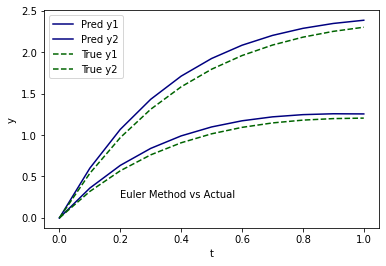
\includegraphics[width=\textwidth]{euler}
				\caption{Approximated $ y_{i} $}
			\end{subfigure}
			\hfill
			\begin{subfigure}[h]{0.47\textwidth}
				\centering
				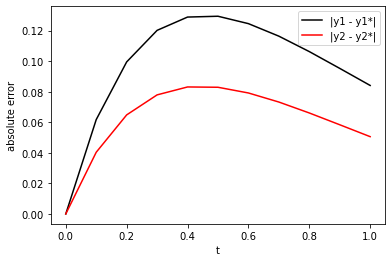
\includegraphics[width=\textwidth]{euler_err}
				\caption{Errors}
			\end{subfigure}
			\caption{Approximation $ y(t) $ obtained by the Euler's Method}
			\label{fig:euler}
		\end{figure}
	
		\begin{figure}[h!]
			\centering
			\begin{subfigure}[h]{0.47\textwidth}
				\centering
				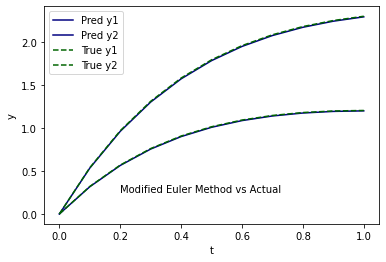
\includegraphics[width=\textwidth]{mod_euler}
				\caption{Approximated $ y_{i} $}
			\end{subfigure}
			\hfill
			\begin{subfigure}[h]{0.47\textwidth}
				\centering
				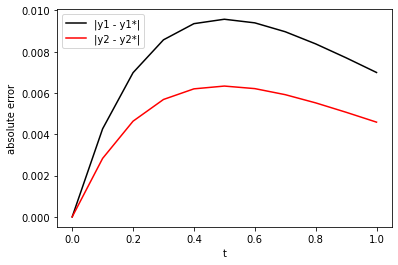
\includegraphics[width=\textwidth]{mod_euler_err}
				\caption{Errors}
			\end{subfigure}
			\caption{Approximation $ y(t) $ obtained by the Modified Euler's Method}
			\label{fig:modeuler}
		\end{figure}
	
		\begin{figure}[h!]
			\centering
			\begin{subfigure}[h]{0.47\textwidth}
				\centering
				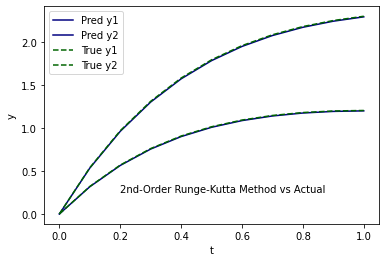
\includegraphics[width=\textwidth]{rk2}
				\caption{Approximated $ y_{i} $}
			\end{subfigure}
			\hfill
			\begin{subfigure}[h]{0.47\textwidth}
				\centering
				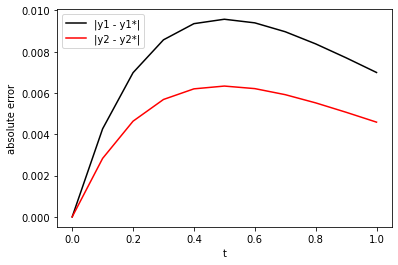
\includegraphics[width=\textwidth]{rk2_err}
				\caption{Errors}
			\end{subfigure}
			\caption{Approximation $ y(t) $ obtained by the \ac{rk2} Method}
			\label{fig:rk2}
		\end{figure}
	
		\begin{figure}[h!]
			\centering
			\begin{subfigure}[h]{0.47\textwidth}
				\centering
				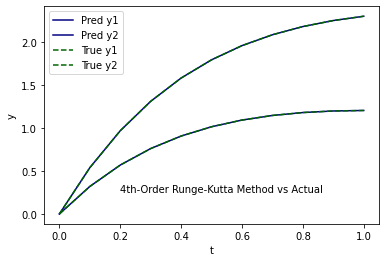
\includegraphics[width=\textwidth]{rk4}
				\caption{Approximated $ y_{i} $}
			\end{subfigure}
			\hfill
			\begin{subfigure}[h]{0.47\textwidth}
				\centering
				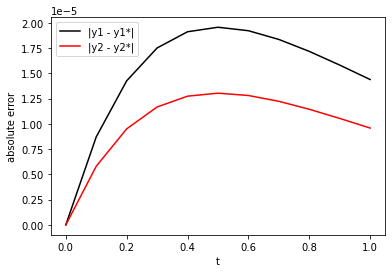
\includegraphics[width=\textwidth]{rk4_err}
				\caption{Errors}
			\end{subfigure}
			\caption{Approximation $ y(t) $ obtained by the \ac{rk4} Method}
			\label{fig:rk4}
		\end{figure}
	
		\begin{figure}[h!]
			\centering
			\begin{subfigure}[h]{0.47\textwidth}
				\centering
				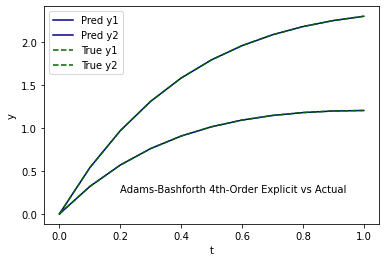
\includegraphics[width=\textwidth]{aexp}
				\caption{Approximated $ y_{i} $}
			\end{subfigure}
			\hfill
			\begin{subfigure}[h]{0.47\textwidth}
				\centering
				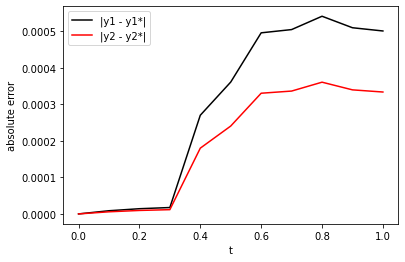
\includegraphics[width=\textwidth]{aexp_err}
				\caption{Errors}
			\end{subfigure}
			\caption{Approximation $ y(t) $ obtained by the Adam Explicit Method}
			\label{fig:aexp}
		\end{figure}
	
		\begin{figure}[h!]
			\centering
			\begin{subfigure}[h]{0.47\textwidth}
				\centering
				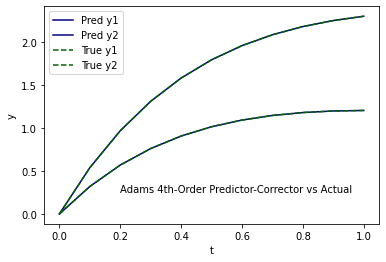
\includegraphics[width=\textwidth]{apc4}
				\caption{Approximated $ y_{i} $}
			\end{subfigure}
			\hfill
			\begin{subfigure}[h]{0.47\textwidth}
				\centering
				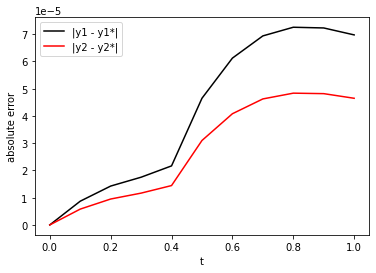
\includegraphics[width=\textwidth]{apc4_err}
				\caption{Errors}
			\end{subfigure}
			\caption{Approximation $ y(t) $ obtained by the Predictor-Corrector Method}
			\label{fig:pc4}
		\end{figure}

\clearpage

	From my python implementation of all methods discussed in \textbf{Chapter 2}. The tables show the timestamps where each $ y_{i} $ approximation is computed and also shows the actual $ y_{i} $ values obtained from (\ref{eq:expsl}). The errors at each timestamp is computed and plotted (right) as well. From the tables and error plots we can clearly see that the Euler is the least accurate method for approximating our \ac{ivp} (\ref{eq:exp}) this is due to the order of error as discussed above. The error of Euler Method accumulates over time thus methods like the Modified Euler is preferred. However, from our numerical experiment we can observe that although the Modified Euler may be a better option compared to the Euler's it also has large errors compared to Runge-Kutta Methods. \ac{rk4} has the best approximation compared to the earlier methods thus it is the most used method in approximation \ac{ivp}. \newline
	As discussed most of our earlier methods only makes one prediction and that is it; the Adams Predictor-Corrector method we discussed, like the name says, first approximates the function with an explicit method and corrects the approximation with an implicit method. Observing the error plot generated by the Adams Predictor Corrector method, the error at each timestamp is lesser and hence more accurate approximations are produced by this method.
	
%%%%%%%%%%%%%%%%%%%%%%%%%%%%%%%%%%%%%%%%%%%%%%

	\backmatter
	
	\addcontentsline{toc}{chapter}{REFERENCES}
	\renewcommand{\bibname}{REFERENCES}
	\bibliography{refs}
	
\end{document}